\subsection{Analog-to-Digital Converter}
\textbf{Teori}

Outputtet fra målinger foretaget på biologiske signaler fremstår som et analogt signal, der er kontinuert i tid og amplitude. For at kunne behandle signalet digitalt, skal signalet konverteres fra analog til digital. Det analoge signal kvantificeres under konverteringen, hvilket gør, at det digitale signal bliver diskret i tid og amplitude \citep{webster1998}. Dette er illusteret på \autoref{fig:ADC_kon}. Konverteringsprocessen består af sampling og kvantificering \citep{morre2003}. 

\begin{figure}[H]
\centering
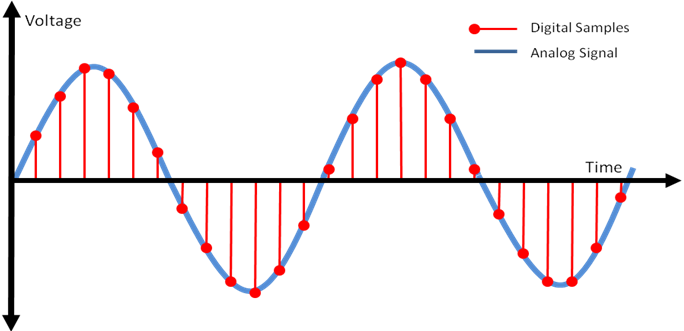
\includegraphics[width=0.7\textwidth]{figures/problemloesning/adc}
\caption{A/D-konvertering fra analog til digital}
\label{fig:ADC_kon}
\end{figure}

\noindent
Samplingsprocessen sker ved diskretisering i tidsdomænet, hvor det kontinuerte signal konverteres til et diskret signal. Det er vigtigt at vælge en passende samplingsfrekvens for at undgå, at information fra det oprindelige signal går tabt \citep{morre2003}. Ved for høj samplingsfrekvens vil en større mængde data opsamles og derved benytte mere plads og processering \citep{wolf2004}. En for lav samplingsfrekvens vil derimod kunne rekonstruere signalet, således kurven ikke kan repræsentere det oprindelige signal, hvilket fremgår som alias \citep{morre2003}. I følge Nyquists sætning er det hensigtsmæssigt, at samplingsfrekvensen er mindst det dobbelte af frekvensen i det oprindelige signal \citep{morre2003}. I praksis anbefales det dog at sample med det ti dobbelte.

Kvantificering sker ved diskretisering af amplituden. Det oprindelige signals amplitudeværdier inddeles ved kvantificering i trin. Værdierne mellem to trin repræsenteres af den samme digitale værdi. Dette gør at flere værdier kan ligge indenfor den samme digitale værdi \citep{morre2003}. Amplitudeniveauer, der er tilgængelige til at repræsentere det analoge signal, determineres af antal bits. En ADC med en opløsning på 12-bit inddeles i ${2}^{12}$, svarende til 4096 niveauer. Den mindste amplitudeniveau som ADC'en kan opnå omtales Least Significant Bit (LSB) og bestemmes ud fra \autoref{equ:LSB}, hvor FSR, hvilket er en betegnelse for Full Scale voltage Range og n antal bits \citep{webster1998, wolf2004}.

\begin{equation} \label{equ:LSB}
LSB=\dfrac{FSR}{2^{12}}
\end{equation}

% = \dfrac{\dfrac{FSR}{{2}^{12}}}
\noindent
Hvis spændingen, der pålægges ADC'en overstiger dens arbejdsområde, vil dette resultere i, at signalet går i mætning \citep{webster1998, wolf2004}.

\vspace{3mm}
\textbf{Krav:}
\begin{itemize}
%\item Skal have en samplingsfrekvens på $100~Hz$
\item Skal sample minimum tre inputs 
%\item Skal have en opløsning på minimum 10 bit
%\item Skal modtage en spændingsforsyning på $XX~V$
%\item Skal have en tolerence på $XX~\%$ (kvatificeringsfejl?)
\end{itemize}

